\documentclass{article}
\usepackage{graphicx}
\usepackage[norsk]{babel}
\usepackage{titlesec}
\usepackage{amsmath}
\usepackage{amssymb}
\usepackage{listings}
\usepackage{xcolor}
\usepackage[utf8]{inputenc}
\usepackage{float}

\title{Diskret Fourier Transform}
\author{Vetle Vatnem , Steffen Gustavsen}

\date{10.04.2025}

\renewcommand{\thesection}{}
\renewcommand{\thesubsection}{}

\lstset{
    language=Python,
    basicstyle=\ttfamily\small,
    keywordstyle=\color{blue},
    stringstyle=\color{red},
    commentstyle=\color{green},
    numbers=left,
    numberstyle=\tiny\color{gray},
    stepnumber=1,
    numbersep=10pt,
    backgroundcolor=\color{white},
    showspaces=false,
    showstringspaces=false,
    showtabs=false,
    frame=single,
    tabsize=4,
    captionpos=b,
    breaklines=true,
    breakatwhitespace=false,
    title=\lstname,
    escapeinside={\%*}{*)},
    morekeywords={*,...}
}


\titleformat{\section}[block]{\normalfont\Large\bfseries}{\thesection}{0em}{}
\titleformat{\subsection}[block]{\normalfont\normalsize\bfseries}{\thesubsection}{0em}{}

\begin{document}
    \maketitle
    \tableofcontents
    \clearpage

\section{Problembeskrivelse}
    Det hele startet med første fourier forelesning med Morten Nome. 
    Et genialt konsept som tar inn et tidsvarierende signal og spytter ut alle frekvenskomponentene.
    Noen uker senere skulle vi lage filter i ESDA1. 
    Oppgaven var å fjerne en pipelyd fra en lydfil.
    Vi kom igang og resultatet ble et filter som var så dårlig at vi tenkte hvem i alle dager hadde brukt noe slikt til dette formålet.
    Videre ble nyskjerrigheten for hvordan de faktisk fjerner slike ulyder stor.
    Etter litt research kom vi over diskret fourier transform eller DFT på kort.
    Uten å forstå så mye ved første øyekast ble oppgaven å forstå konseptet, utlede og implementere en DFT på enklest mulig måte.
    Prosjektet har en baktanke. Det er å kunne viderereutvikle programmet for å bli brukt videre i skolegangen.
    Derfor er det også et enkelt grafisk brukergrensesnitt på porteføljen.

\section{Diskret fourier transform}
    En diskret fourier transform er en transform som tar inn et diskretisert signal og spytter ut frekvenskomponentene.
    Måten dette blir kalkulert på er i bunn å grunn en hel haug med prikkprodukter. Jo flere samples jo flere prikkprodukt må datamaskinen gjøre og lagre.
    Videre blir det vist at antall samples er viktig for både hvilke frekvenser en får ut og effektiviteten til programmet.
    
    \subsection{En utledning}
        Det finnes flere metoder for å utlede diskretfourier transform. 
        Den enklesete er vel å diskretisere den kontinuerlige fouriertransformen, men det er jo ufattlig kjedlig og gir dårlig læringsutbytte.
        Derfor ble det bestemt at en annen metode skulle brukes.

        \subsubsection{Basis}
            Hele fourier geiene handler om et indreprodukt mellom signalet og en eller annen basis.
            Basisen inneholder såklart alle de forskjellige frekvensene vi tester om finnes i signalet.
            Dermed blir første byggestein å finne en basis for et vektorrom vi kan projisere signalet ned på.
            Vi starter med en enkel kompleks funksjon som har amplitude \(1\) som vist i figuren under.

            \begin{figure}[H]
                \centering
                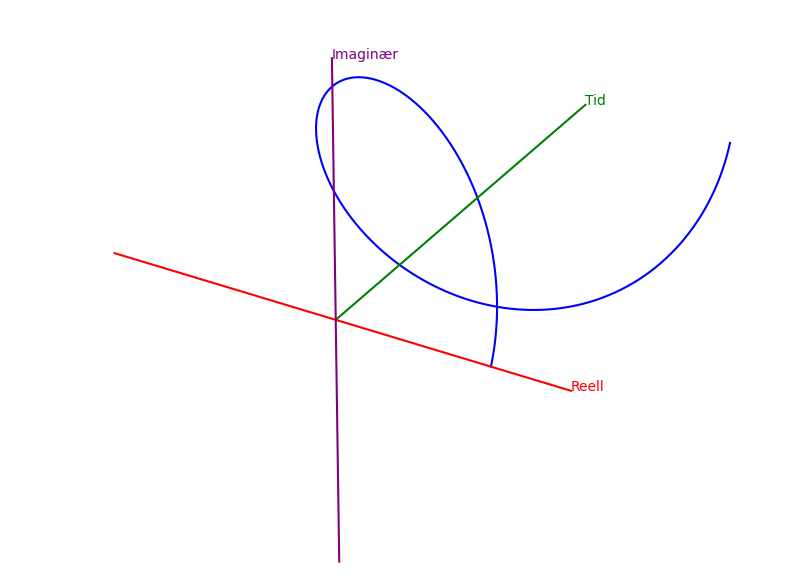
\includegraphics[width = 0.8\textwidth]{Bilder/BasisEksempelFunksjon.png}
                \caption{\(f(t) = cos(t) + isin(t)\), \(i = \sqrt{-1}\)}
            \end{figure}

            Deretter sampler vi signalet 8 ganger med like mellomrom på tidsaksen og ser nærmere på resultatet vi får i det komplekseplanet.

            \begin{figure}[H]
                \centering
                \begin{minipage}[c]{0.45\textwidth}
                    \centering
                    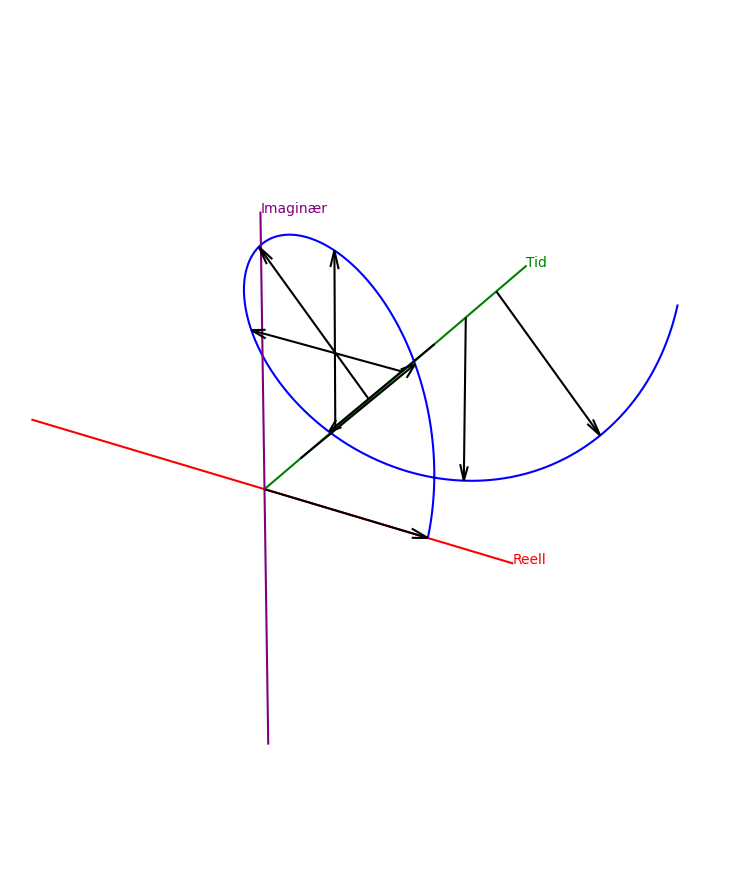
\includegraphics[width = 1\textwidth]{Bilder/BasisEksempelFunksjonMedVektorer.png}
                    \caption{\(f(t) = cos(t) + isin(t)\), \(i = \sqrt{-1}\)}
                    \label{fig:BasisEksempelFunksjonMedVektorer}
                \end{minipage}
                \hfill
                \begin{minipage}[c]{0.45\textwidth}
                    \centering
                    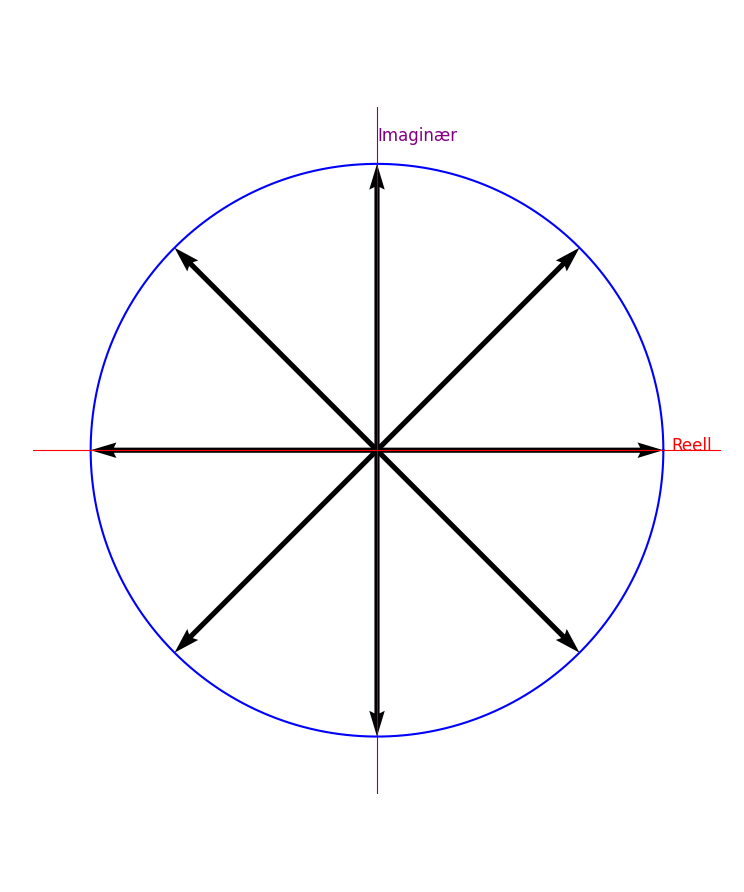
\includegraphics[width = 1\textwidth]{Bilder/KomplekseplanetMedVektorer.png}
                    \caption{}
                \end{minipage}
            \end{figure}

            Når vi nå analyserer vektorene i det komplekse planet blir det klart at funksjonen er \(2\pi\) periodisk.
            Det som også er verdt å merke er at vinkelen mellom den reelle aksen og vektorene tilsvarer en eller annen vinkelfrekvens \(\omega\).
            Denne påstanden kan enkelt ses i figur \ref{fig:BasisEksempelFunksjonMedVektorer} siden en vinkel i det komplekseplanet tilsvarer en vinkel per tidsenhet i figuren.
            Dermed kan man kalle denne for vinkelfrekvens \(\omega\). 
            Siden signalet er \(2\pi\) periodisk i det komplekseplanet ser vi at \(\omega_0 = -\frac{2\pi}{N}\) der \(N\) er antall samples.
            Der \(\omega_0\) er vinkelenendringen per sample altså den korteste vinkelhastigheten.
            Nå er det grunn til å lure på hvorfor \(\omega_0\) er negativ og det er fordi vi beveger oss med klokken på sirkelen som gir negative vinkler.
            Med denne informasjonen kan vi gi et utrykk for hver vektor i funksjonen med hjelp av Eulers formel og samtidig legge til \(n\) for bevegelsen langs tidsaksen.

            \[
                f_k(n) = e^{-i\frac{2\pi kn}{N}} \hspace{2cm} k,n \in \{0 , N-1\} 
            \]

            En måte å tenke på denne ligningen er at vi tar \(N\) vektorer og fordeler de med lik vinkel mellom dem på distansen \(k\) ganger omkretsen på sirkelen som er en enhetssirkel.
            Ut fra dette kan man se at \(n\) representerer et tidssteg på tidsaksen. 
            Den er bundet til samplefrekvensen.
            Da har vi at formelen over er \(k\) det som utgjør indeksen for hvilken frekvens det er og \(n\) hvilket tidsteg. Dette blir viktig senere.
        
        \subsubsection{Indreprodukt}
            Nå er vi interesert i hvor mye av hver \(k\)-te frekvens det er i et gitt signal \(x(t)\). 
            La oss si at \(x(t)\) har periode \(T\) og blir samplet \(N\) ganger på den perioden.
            Lille \(n\) representerer dermed indeksen for hvert tidssteg og vi kan skrive \(x(n)\) der verdien av \(x(n)\) er et reelt tall og \(n \in \{0,N-1\}\).
            Dermed kan vi definere et indreprodukt der vi gjør om \(x(n)\) og \(f_k(n)\) til vektorer.

            \[
            \vec{x} =
            \begin{bmatrix}
            x(0) \\ x(1) \\ x(2) \\ . \\ . \\ . \\ x(N-1)
            \end{bmatrix}
            =
            \begin{bmatrix}
            x_0 \\ x_1 \\ x_2 \\ . \\ . \\ . \\ x_{N-1}
            \end{bmatrix}
            \quad , \quad
            \vec{f_k} =
            \begin{bmatrix}
            f_k(0) \\ f_k(1) \\ f_k(2) \\ . \\ . \\ . \\ f_k(N-1)
            \end{bmatrix}
            =
            \begin{bmatrix}
                f_0 \\ f_k \\ f_{k2} \\ . \\ . \\ . \\ f_{k(N-1)}
            \end{bmatrix}
            \]

            \[
                \vec{f_k}^T\vec{x} = \sum_{n = 0}^{N-1}f_{kn}x_n = N\hat{x}_k
            \]

            Da deler vi på \(N\) og får følgende formel for den \(k\)-te frekvensen.

            \[
                \hat{x_k} = \frac{1}{N}\sum_{n = 0}^{N-1}f_{kn}x_n = \frac{1}{N}\sum_{n = 0}^{N-1}x_ne^{-\frac{i2\pi kn}{N}}
            \]

    \subsection{Implementering}
        For å finne alle \(\hat{x_k}\) ser man raskt at dette kan skrives slik.

        \[
            \vec{\hat{x}} =
            \begin{bmatrix}
                \sum_{n = 0}^{N-1}x_n \cdot 1 \\ \sum_{n = 0}^{N-1}x_n \cdot e^{-\frac{i2\pi n}{N}} \\ \sum_{n = 0}^{N-1}x_n \cdot e^{-\frac{i2\pi 2n}{N}} \\ . \\ . \\ . \\ \sum_{n = 0}^{N-1}x_n \cdot e^{-\frac{i2\pi (N-1)n}{N}}
            \end{bmatrix}
        \]
        
        Siden vi har en sum e hver rad av vektoren kan dette skrives som en matrise-vektor multiplikasjon slik.
        
        \[
            \vec{\hat{x}} = \frac{1}{N}\boldsymbol{F}\vec{x} \\
        \]
        
        \[
            \boldsymbol{F} = 
            \begin{bmatrix}
            1 &       1                     &        1                  & . & . & . & 1                       \\ 
            1 & e^{-\frac{i2\pi}{N}}    & e^{-\frac{i4\pi}{N}}    & . & . & . & e^{-\frac{i2\pi (N-1)}{N}}    \\ 
            1 & e^{-\frac{i4\pi}{N}}    & e^{-\frac{i8\pi}{N}}    & . & . & . & e^{-\frac{i4\pi (N-1)}{N}}    \\ 
            . &       .                 &         .               & . &   &   & .                             \\ 
            . &       .                 &         .               &   & . &   & .                             \\
            . &       .                 &         .               &   &   & . & .                             \\
            1 & e^{-\frac{i2\pi (N-1)}{N}} & e^{-\frac{i4\pi (N-1)}{N}}                       & . & . & . & e^{-\frac{i2\pi(N-1)^2}{N}}                            \\
            \end{bmatrix}
        \]

        Dermed har vi en metode som kan implementeres på en datamaskin. Det ble laget en klasse med navn matrise der det ble overlastet operatoerer for ganging med både vektorer og matriser.
        Oppbyggningen til matrise klassen kan ses i filen Matrix.h. I filen Fourier.h blir matrisen \(\boldsymbol{F}\) laget og lagret.
        \(x(t)\) blir lagt inn via en CSV fil som leses av via input i grafikk vinduet. For å finne ut av hvilken frekvens som gir utslag må man gange \(\frac{k}{N}\) med samplefrekvensen.
        Derfor er samplefrekvensen viktig fordi den bestemmer hvor liten frekvens som er den laveste.
        Det er derfor også viktig at samplefrekvensen er høyere enn fundamentalfrekvensen til signalet.
        Den må være minst dobbelt så stor slik at samplefrekvensen får tre punkter i en periode av fundamentalfrekvensen og dermed utelukker frekvenser som har mindre frekvens enn fundamentalfrekvensen.
        Ut fra matrisen over kan det også ses at vektoren \(\vec{\hat{x}}\) blir speilet om \(\frac{N}{2}\) og er komplekse tall.
        De frekvensene over \(\frac{N}{2}\) er noe som heter aliasing 
        Siden signalene vi har tenkt å stappe inn i denne DFTen er reelle blir amplituden \(2|\hat{x_k}|\) der \(k\) er indeksen i vektoren \(\vec{\hat{x}}\). 
        Det kommer av Eulers formel og summeringen av komplekskonjugerte som gjør at de imaginære bitene nuller hverandre ut og 

        \[
            cos(t) = \frac{1}{2}\left(e^{it} + e^{-it}\right) \quad , \quad sin(-t) = -sin(t)
        \]

        Lengre ned får man instuksjoner om å gange med 2 for å finne amplituden og det er på grunn av den første likningen over. 
        Vi summerer alle produktene som gir oss en av de to i leddene over som vil si at vi på gange med 2 for å få amplituden eller hente ut de komplekskonjugerte, ta absoluttverdien og legge de sammen.
        Grunnen for at dette skjer er fordi \(\text{cos}(-t) = \text{cos}(t)\). 
    
    \section{Brukergrensesnitt}
        Brukergrensesnittet er ikke helt ferdig enda men er på god vei. Vi ble dessverre ikke helt ferdig.
        Uansett er det som sagt et prosjekt vi har tenkt til å jobbe med videre og muligens benytte i skolesammenheng.

        \subsection{Hvordan kjøre programmet.}
            Når man skal kjøre programmet er det viktig å trykke CTRL+F5 slik at den ikke går inn i debugmode. 
            Det er fordi den kan kaste en int3 error som ikke er reell. 
            Uansett. 
            Siden GUI ikke er helt ferdig enda er det kommentert ut en kodesnutt i main som skriver ut en fourierkoefissient til terminalen.
            Fouriervektoren kan være flere 1000 elementer lang så det er nødvendig skrive ut de frekvensene man er interesert i. 
            Det gjør man ved å bruke følgende formel.
            
            \[
                k = \frac{fN}{S_f}
            \]

            Der \(k\) er indeksen i fourier-vektoren, \(N\) er antall samples, \(f\) er frekvensen du vil skrive ut amplituden til og \(S_f\) er sample frekvensen.
            Når det kommer til kjøring av programmet er det viktig at datamaskinen har en del tilgjengelig minne(RAM) om \(N\) er veldig stor så vær obs på det.
            Det er et problem vi skal fikse med implementering av en FFT algoritme istedenfor å kalkulere hele DFTen ut fra definisjonen. Fin sommerjobb.
            Her er en bruksanvisning for de som liker det.

            \begin{itemize}
                \item Funksjonen A.getFourierCoefficients(), gir vektoren med Fourierkoeffisientene
                \item Finn elementet $k$ som gir frekvensen $f$ med formelen: $k = \frac{Nf}{S_f}$, hvor $S_f$ er samplefrekvens og $N$ er antall elementer. Frekvensen og samplefrekvensen til signalet er gitt i tittelen til CSV-filene som ligger repoen.
                \item Finn amplituden til et element ved å ta $|\hat{x}_k|2$.
                \item Lagre ønsket CSV-fil.
                \item Kompiler (Ctrl+F5).
                \item Legg inn path til CSV-fil i tekst inputfeltet.
                \item Trykk på "Load" knappen (det kan ta litt tid hvis. Hvis man er usikker på om den er ferdig kan man se på minnebruken til programmet som kjører i taskmanager. Når det nærmer seg normalt nivå er den ferdig).
                \item Trykk på "Quit" knappen og les av resultetene i terminalen.
            \end{itemize}
            
\end{document}